\chapter{Hardware}\label{ch:hw}

\section{Components}
The aim of this section is to describe in detail the parts and chosen components for this design. Most of these components are quite common among other research projects, and some of them are custom parts.

There are two drone models that were developed for this project, models A and B. 

First, the Table \ref{tab:comp_common} shows the common components for both models. Then, the Table \ref{tab:comp_AB} shows the additional components and to which model they belong to. Finally, the Table \ref{tab:comp_custom} lists the parts that were specifically designed for this project and were done externally.

% mention also adapters and other cablesthat were used during the development?

% Please add the following required packages to your document preamble:
% \usepackage[table,xcdraw]{xcolor}
% If you use beamer only pass "xcolor=table" option, i.e. \documentclass[xcolor=table]{beamer}
\begin{table}[H]

\centering
    \caption{Common components for all models}
    \label{tab:comp_common}
    
\begin{tabular}{lll}
\hline
\rowcolor[HTML]{FFFFFF} 
\multicolumn{1}{|l|}{\cellcolor[HTML]{FFFFFF}Category} & \multicolumn{1}{l|}{\cellcolor[HTML]{FFFFFF}Component} & \multicolumn{1}{l|}{\cellcolor[HTML]{FFFFFF}Description}  \\ \hline
\rowcolor[HTML]{9AFF99} 
Sensors                                                & FTDI LC231X                                            & UART-USB adapter                                                                                                    \\
\rowcolor[HTML]{9AFF99} 
                                                       & FlySky FS-iA6                                          & Receiver                                                                                                             \\
\rowcolor[HTML]{9AFF99} 
                                                       & Turnigy TGY-i6                                                       & Transmitter                                                                                                          \\
\rowcolor[HTML]{9AFF99} 
                                                       & MPU-6050                                               & IMU                                                                                                                  \\
\rowcolor[HTML]{9AFF99} 
                                                       & MS5611                                                 & Barometer                                                                                                            \\
\rowcolor[HTML]{9AFF99} 
                                                       & M8N 8M 8N                                              & GPS and compass                                                                                                      \\
\rowcolor[HTML]{9AFF99} 
                                                       & 3DR Radio 433MHZ                                       & Telemetry                                                                                                            \\
\rowcolor[HTML]{FFFFC7} 
Body                                                   & F450 frame                                             & Frame                                                                                                                \\
\rowcolor[HTML]{FFFFC7} 
                                                       & ZIPPY 2200mAh 3s 40c                                   & Lipo battery                                                                                                         \\
\rowcolor[HTML]{CBCEFB} 
Development                                            & Altera de10-nano                                       & FPGA Board                                                                                                          
\end{tabular}
\end{table}

% Please add the following required packages to your document preamble:
% \usepackage[table,xcdraw]{xcolor}
% If you use beamer only pass "xcolor=table" option, i.e. \documentclass[xcolor=table]{beamer}
\begin{table}[H]

\centering
    \caption{Different components for each model}
    \label{tab:comp_AB}
    
\begin{tabular}{lll}
\hline
\rowcolor[HTML]{FFFFFF} 
\multicolumn{1}{|l|}{\cellcolor[HTML]{FFFFFF}Category} & \multicolumn{1}{l|}{\cellcolor[HTML]{FFFFFF}Component} & \multicolumn{1}{l|}{\cellcolor[HTML]{FFFFFF}Description} \\ \hline
\rowcolor[HTML]{9AFF99} 
Model-A                                                   & Readytosky 2212                                           & Set of 4 motors + ESCs                                                                                                        \\
\rowcolor[HTML]{FFFC9E} 
Model-B                                                   & AirGear 450                                            & Set of 4 motors + ESCs                                                                                                       \\
\rowcolor[HTML]{FFFC9E} 
                                                    & GMP v1.0 XT                                            & Power module                                                                                                        
\end{tabular}
\end{table}

% Please add the following required packages to your document preamble:
% \usepackage[table,xcdraw]{xcolor}
% If you use beamer only pass "xcolor=table" option, i.e. \documentclass[xcolor=table]{beamer}
\begin{table}[H]

\centering
    \caption{Custom components for all models}
    \label{tab:comp_custom}
    
\begin{tabular}{lll}
\hline
\rowcolor[HTML]{FFFFFF} 
\multicolumn{1}{|l|}{\cellcolor[HTML]{FFFFFF}Category} & \multicolumn{1}{l|}{\cellcolor[HTML]{FFFFFF}Desciption} & \multicolumn{1}{l|}{\cellcolor[HTML]{FFFFFF}Designed with} \\ \hline
\rowcolor[HTML]{9AFF99} 
Electronics                                            & PCB                                                     & DipTrace                                                   \\
\rowcolor[HTML]{FFFC9E} 
Mechanics                                                   & Cover                                                   & SolidWorks 2019                                            \\
\rowcolor[HTML]{FFFC9E} 
                                                       & FPGA-Frame attachment                                   & TinkerCAD                                                 \\
\rowcolor[HTML]{FFFC9E} 
                                                       & GPS-Cover attachment                                   & TinkerCAD                                                                                           
\end{tabular}
\end{table}


In case of the model A, most of its components can be bought together as a kit for the Ardupilot F450 Quadcopter \cite{bib:drone_Kit}, which includes the frame, the motors, ESCs, transmitter, receiver, and the GPS-compass.

%% ========================== MECHANICS ==========================
\section{Mechanical design}\label{sec:hw_mec}

\subsection{Assembly}

For both models, the drone type is a quad-copter, with the dimensions of 363mm x 363mm and 152.54mm height. The total weight of the drone with all the components mounted (except the battery) is 1.110kg for the Model-A and 1.170kg for Model-B. Inside the frame, a custom part attaches the FPGA to the top of the frame.

The main mechanical assembly can be seen in Figure \ref{fig:hw_assembA}, which shows the frame, motors, propellers and cover:

\begin{figure} [H]
    \centering
    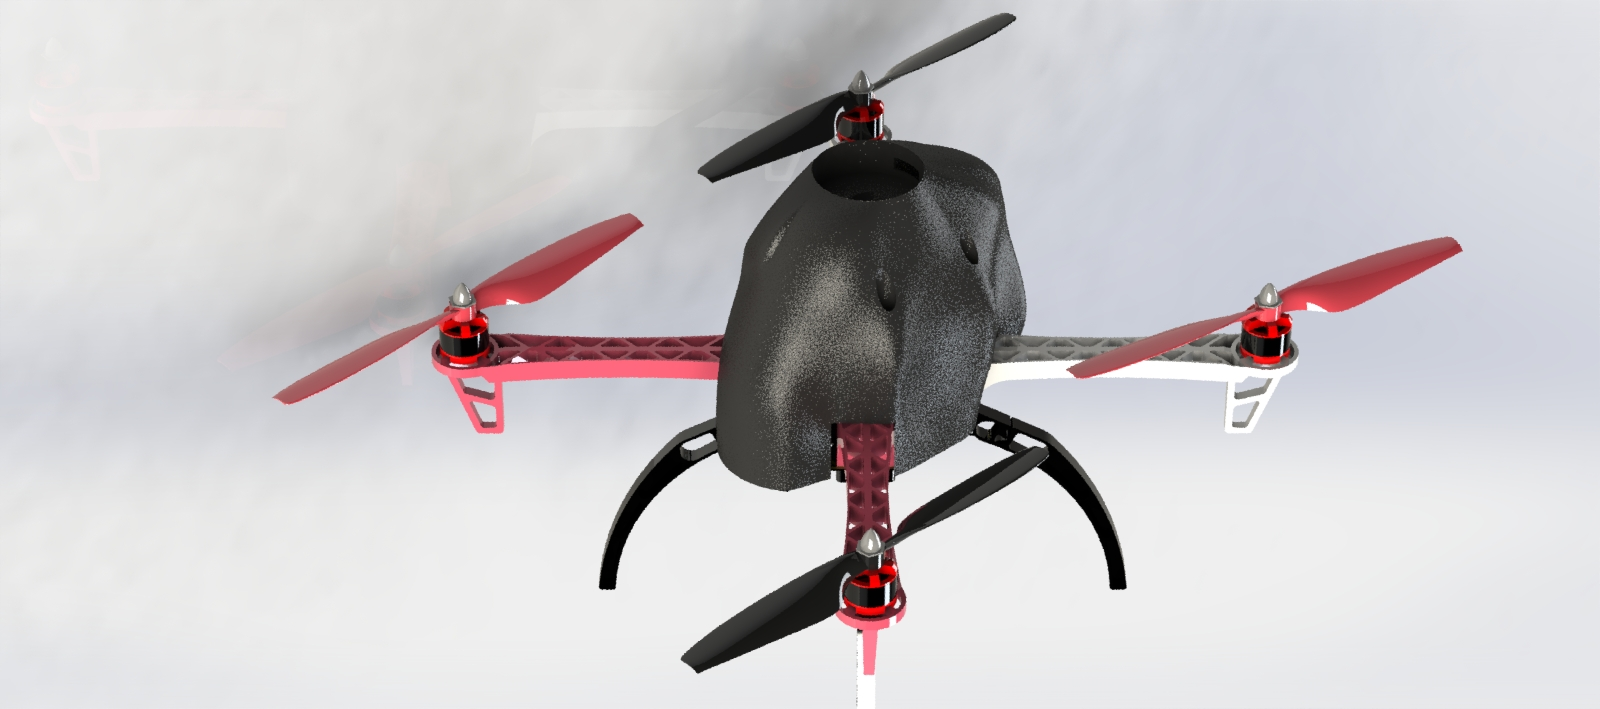
\includegraphics[width=\textwidth]{Figures/hardware/render_assemblyA.JPG}
    \caption{Model A assembly in SolidWorks. Frame, motors and propellers original design from Alejandro Llorente \cite{bib:droneCAD}}
    \label{fig:hw_assembA}
\end{figure}

Inside the frame and cover, the space is distributed as shown in Figure \ref{fig:hw_space}. In case of model B, the only addition to this is that the power module is inside the bottom level, sharing space with the battery: 

\begin{figure} [H]
    \centering
    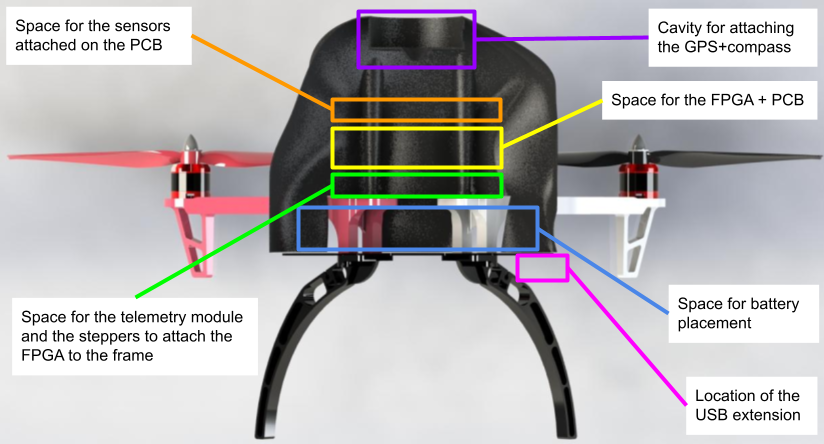
\includegraphics[width=\textwidth]{Figures/hardware/drone_spaces.png}
    \caption{Cut side view of the space distribution for the components inside the Model A assembly. Notice that "Location of the USB extension" refers to a cable extension connected to the UART-USB adapter (located on top of the PCB), so it is possible to download the flight controller application without removing the cover. Also notice that the telemetry module is attached on the same level as the steppers due to its antenna size and therefore it does not fit on top of the PCB as the rest of the sensors.}
    \label{fig:hw_space}
\end{figure}


\subsection{Custom body parts}

As seen on the Table \ref{tab:comp_custom}, some components of the project are custom and therefore, exclusively designed for this project. This subsection describes the mechanical parts, which are the cover, the GPS attachment the FPGA-Frame attachment. All three parts got done with the 3D printers at Aalborg University.

As an overview, the cover and the FPGA-Frame parts are attached to the top of the frame. In case of the GPS attachment, it is a top that holds the GPS on the cover. 


First, the FPGA-Frame attachment is a support part that allows to attach the FPGA to the body, since the drone frame was meant to be used with another controller. This attachment part is shown in Figure \ref{fig:hw_fpgaBase}  and its size is of 70.59mm x 109.54mm and a thickness of 2 mm.

\begin{figure}[!htb]
    \centering
    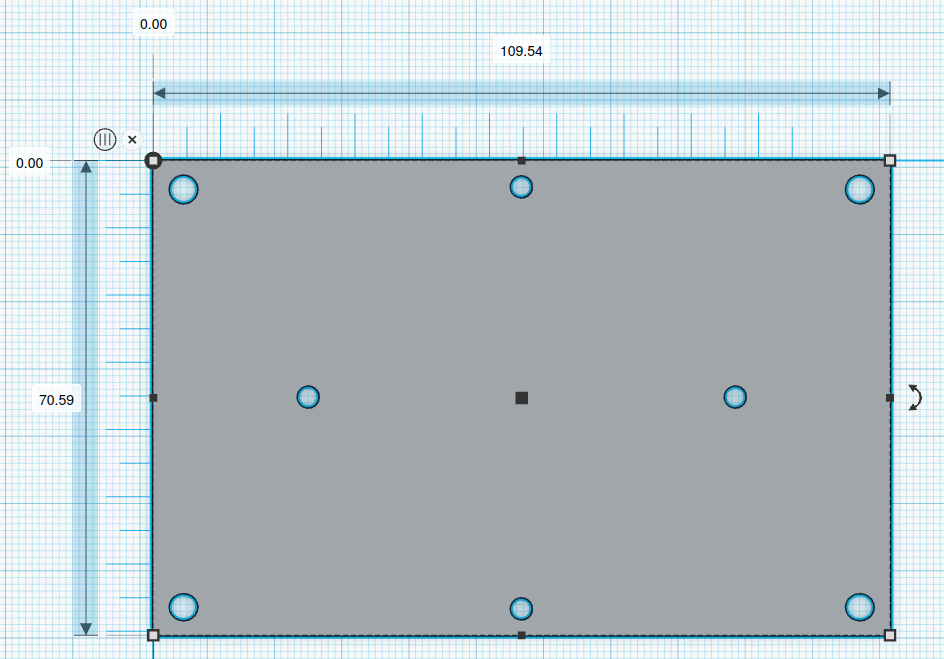
\includegraphics[width=\textwidth]{Figures/hardware/fpga_attachment.png}
    \caption{FPGA-Frame attachment custom part. The four holes on the corners are for the FGPA and the four holes on the center are for the body frame. All screws and steppers are size M3. The length for the steppers is 6mm.}
    \label{fig:hw_fpgaBase}
\end{figure}


Secondly, the cover protects the components and the board from possible impacts and other unexpected events during the fly. The cover is shown in Figure \ref{fig:hw_cover}, which has a size of 194.81mm x 131.46mm, a total height of 158.84mm and a thickness of 0.75mm:

\begin{figure}[!h]
    \centering
    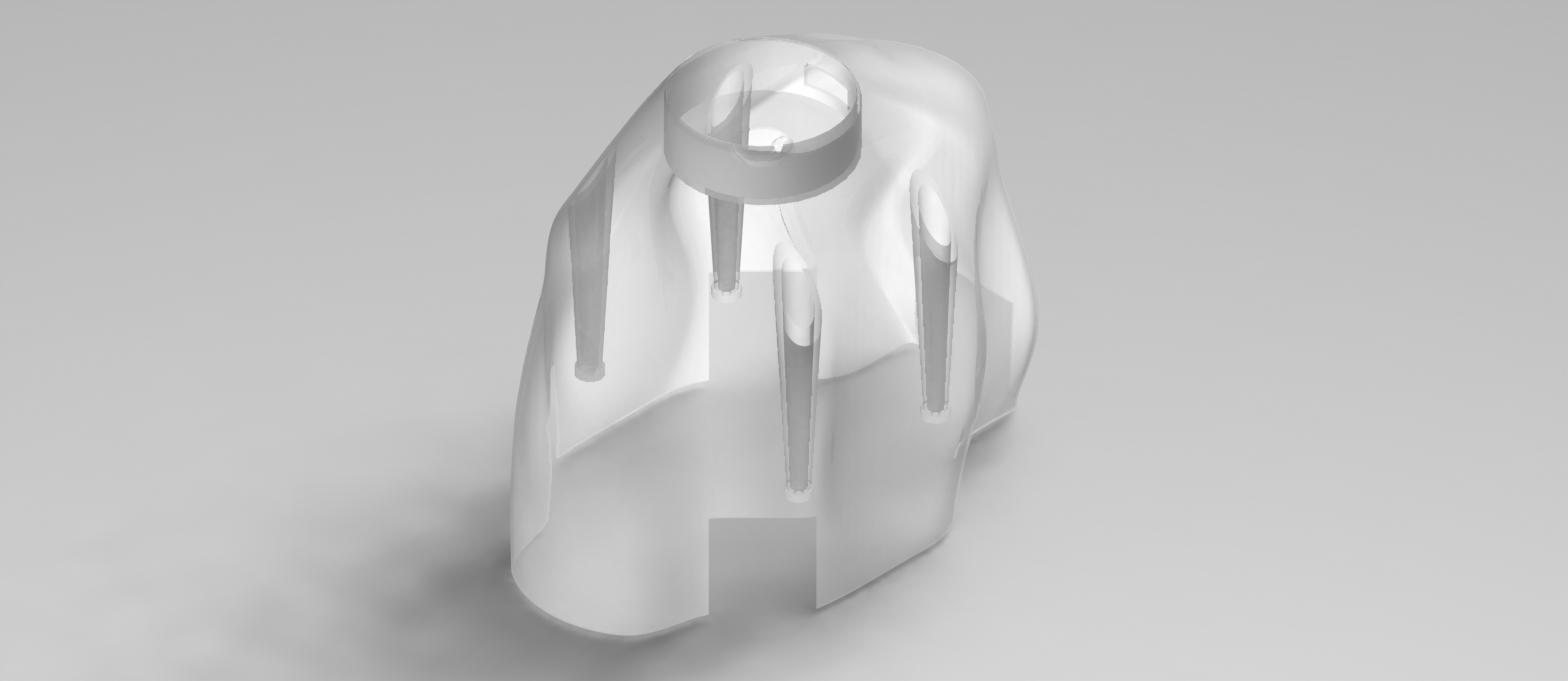
\includegraphics[width=\textwidth]{Figures/hardware/cover_transPlastic.JPG}
    \caption{Cover rendered using a transparent plastic material. This shows the legs for the attaching the cover to the frame (using screws M2), the cavity for the GPS on the top and the holes on the bottom part for the arms and the battery.}
    \label{fig:hw_cover}
\end{figure}

Finally the GPS-Frame attachment is a 12mm x 12mm and 14mm height that is placed inside the cover, on the bottom whole for the GPS and attach it to the frame with a screw as shown in Figure \ref{fig:hw_gps}.

\begin{figure}[!ht]
    \centering
    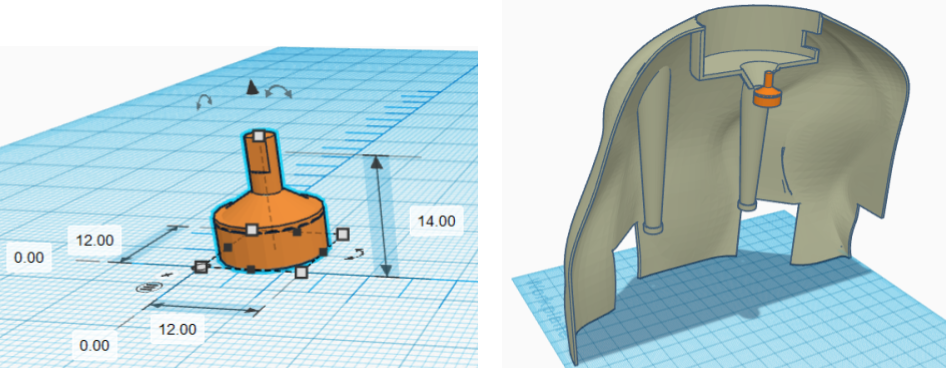
\includegraphics[width=\textwidth]{Figures/hardware/GPS_Attach.png}
    \caption{GPS-Frame attachment dimensions (left) and its placement in the cover (right). This part is held inside the GPS with a screw M1.}
    \label{fig:hw_gps}
\end{figure}

\vfill % <- use this to avoid big blank spaces
\clearpage
%% ========================== ELECTRONICS ==========================
\newpage
\section{Electrical and electronics design}\label{sec:hw_elec}

\subsection{Design overview}
In both modes A and B, the battery provides a power supply of +12V and it is connected to the ESCs. Also both models have in common that all the other components and FPGA board require a power supply for +5V.
In case of Model-A, the +5V supply comes from the ESCs. However, in case of Model-B the +5V is given by the power module, which is between the battery and the the ESCs. 

The next two Figures \ref{fig:hw_modelA} and \ref{fig:hw_modelB} show the hardware diagrams for both models, including the power distribution, the components listed previously in Tables \ref{tab:comp_common} and \ref{tab:comp_AB} and the type of communication between the components and the FPGA.

\begin{figure}[!htb]
    \centering
    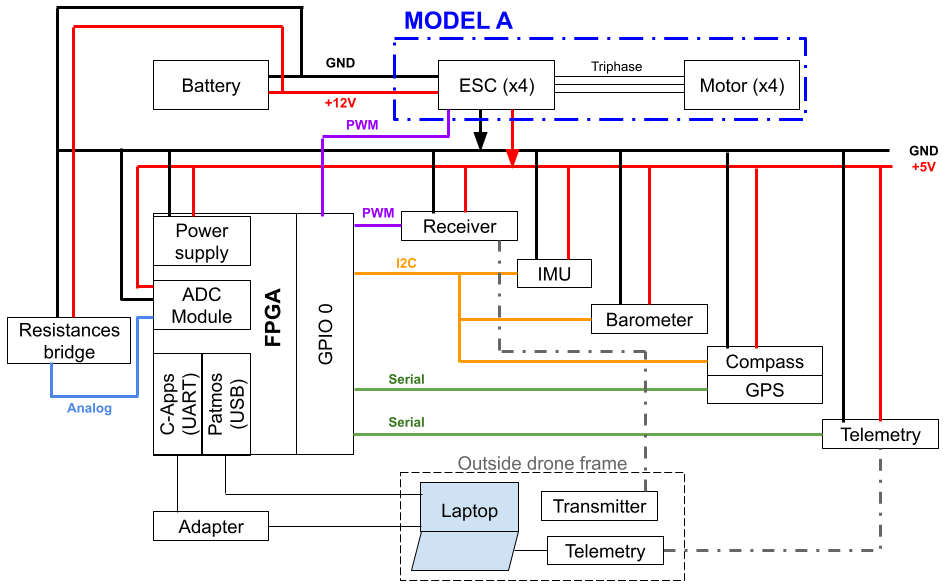
\includegraphics[scale=0.42]{Figures/hardware/Hardware_diagramA_ADC.png}
    \caption{Hardware diagram overview for Model-A.}
    \label{fig:hw_modelA}
\end{figure}

\begin{figure}[!htb]
    \centering
    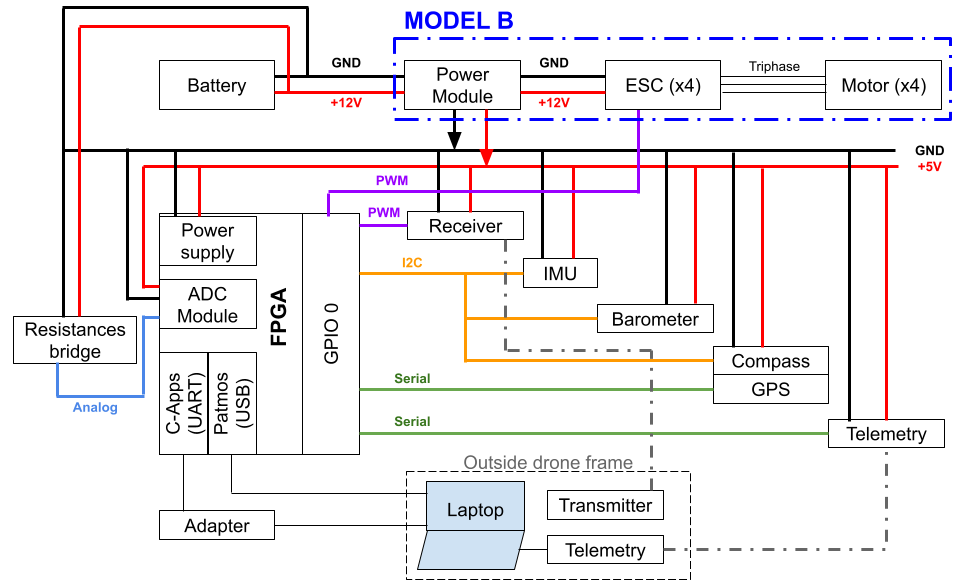
\includegraphics[scale=0.42]{Figures/hardware/Hardware_diagramB_ADC.png}
    \caption{Hardware diagram overview for Model-B.}
    \label{fig:hw_modelB}
\end{figure}

Low-level characteristics of these designs to take into account for the FPGA set-up:
\begin{itemize}
    \item PWM signals from the receiver are inputs, PWM signals going to the ESCs are outputs.
    \item Serial devices have an input (RX) and an output (TX).
    \item The ADC module is a SPI LTC2308 module already integrated within the FPGA. The analog input that it can read is on differential configuration, which has a range of $[+2.048,$ $-2.048]V$. The resistances bridge re-scales the amplitude of the battery $[+11.4,0]V$ to $[+1.937,0]V$, which is safer for the module, as shown in Figure \ref{fig:hw_adc}.
\end{itemize}

\begin{figure}[H]
    \centering
    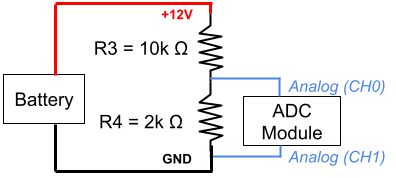
\includegraphics[scale=0.45]{Figures/hardware/resistances_bridge.png}
    \caption{Resistances bridge for the ADC module input. Original design and names from Joop Brokking \cite{bib:brooking}.}
    \label{fig:hw_adc}
\end{figure}

\subsection{FPGA and PCB}

Going into more detail on the electronics design, the following Figure \ref{fig:hw_pins} shows the pins connection of the FPGA to the devices. This diagram is the same for both models.

\begin{figure}[!ht]
    \centering
    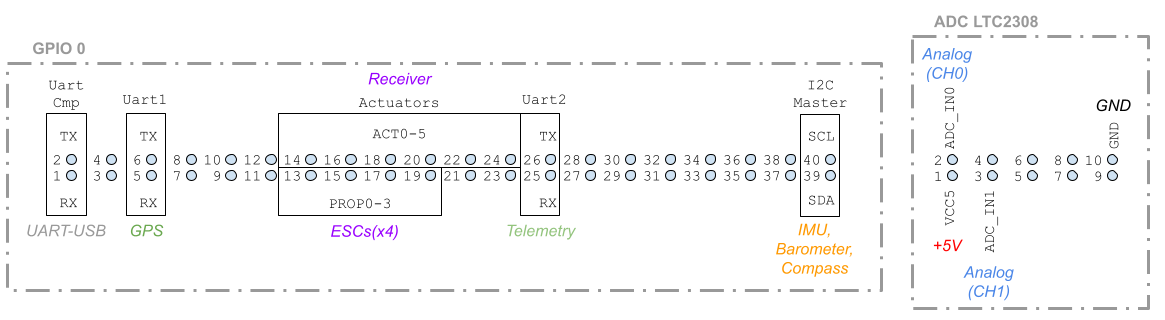
\includegraphics[width=\textwidth]{Figures/hardware/FPGA_pins_ADC.png}
    \caption{De10-Nano pins connection to the components. The pins on use have their name next to them and they are contained in a box with the name of the device type (written in black: UART1, I2CMaster,...) and what physical component is (written in the same color as in the global diagram in Figures \ref{fig:hw_modelA} and \ref{fig:hw_modelB}: receiver, GPS, compass,...)}
    \label{fig:hw_pins}
\end{figure}

In order to simplify the assembly and reduce the amount of wiring in the frame, a PCB was designed for this project.
The PCB was designed in an open source software called DipTrace using the mechanical layout of De10-Nano board as shown in Fig. \ref{fig:mech_layout}. It was designed as a shield for the FPGA. The shield is attached to the GPIO pins and the analog pins of the FPGA and it is fixed by bolting it on 4 corners. The complete PCB design can be seen in Fig. \ref{fig:pcb}.  The PCB remains the same for both model drones i.e. Model A and B and the only difference being that in the model B, the 5V power comes from a power module and it slots into Model B pins in the PCB shield. Whereas in a Model A, the power is directly received from ESC through a Battery Elimination Circuit (BEC). The convention for the pin hole design is such that, the square pins are for power and the circular holes are for other pins.

\begin{figure}[!htb]
    \centering
    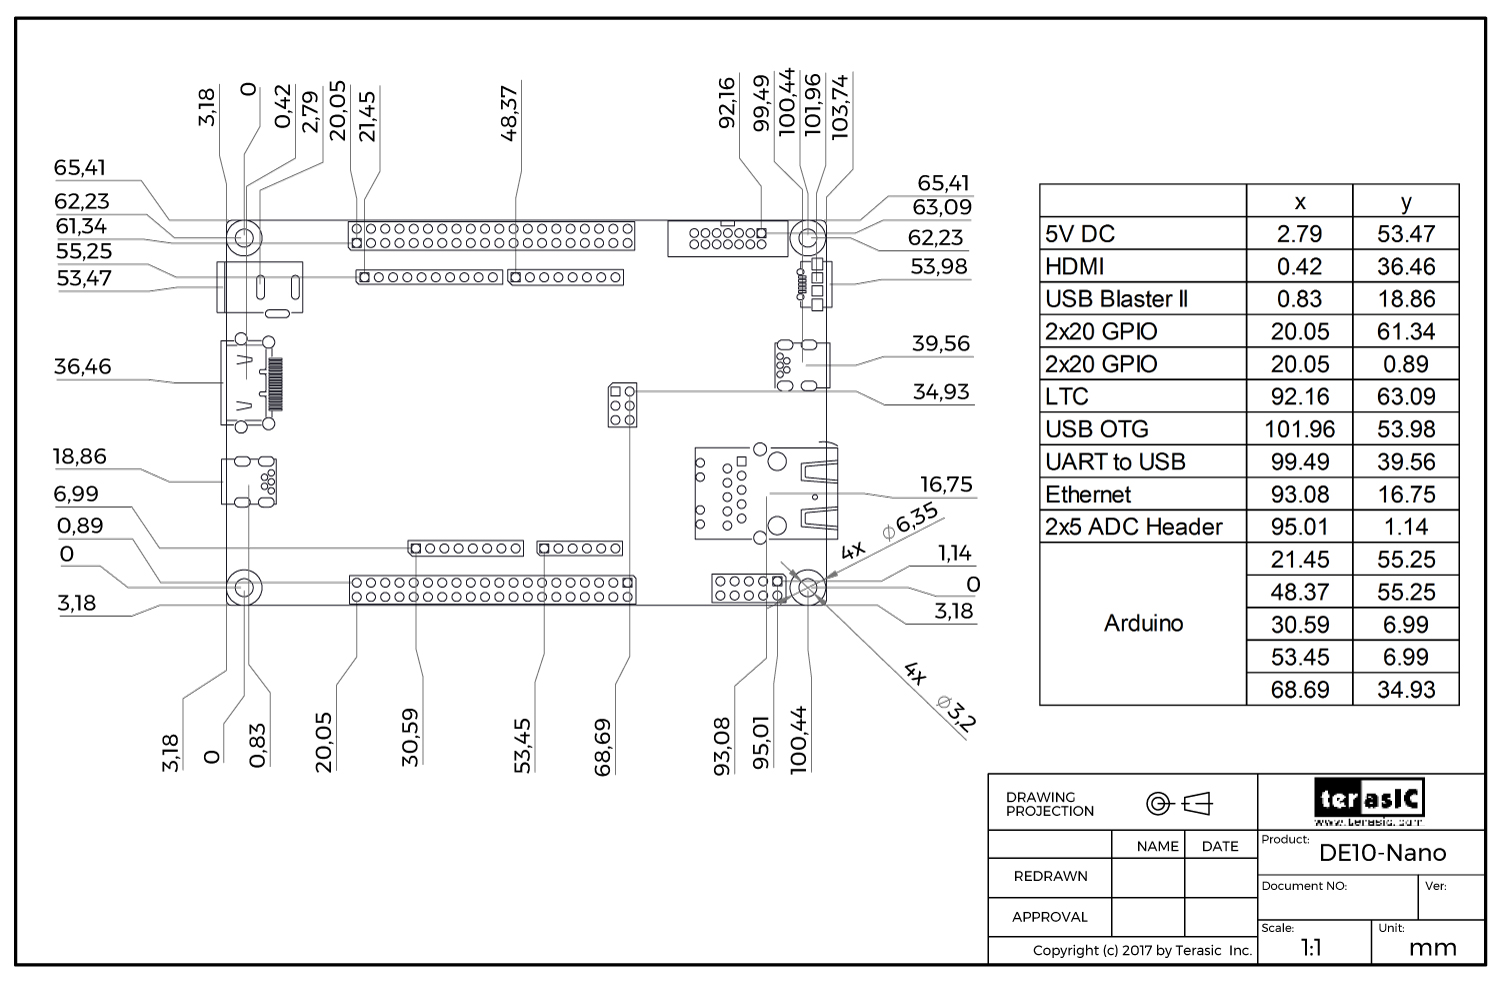
\includegraphics[width=\textwidth]{Figures/hardware/mechanical_layout.jpg}
    \caption{The mechanical layout of the De10-Nano board \cite{bib:fpga_layout}.}
    \label{fig:mech_layout}
\end{figure}

\begin{figure}[!htb]
    \centering
    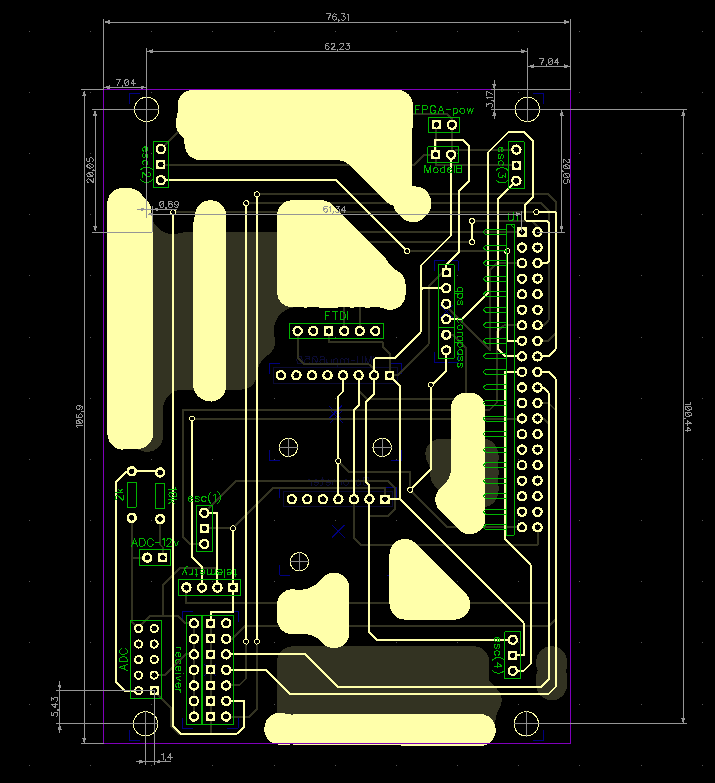
\includegraphics[width=\textwidth]{Figures/hardware/PCB_diptrace.PNG}
    \caption{Top view of the PCB shield designed for de10-nano board.}
    \label{fig:pcb}
\end{figure}
